pakkediagram
\todo{I 4+1 arkitekturen kan det logiske view repræsenteres med et pakkediagram.}
Figur~\ref{fig:packageDiagram} viser projektets pakkediagram. Diagrammet viser systemets pakker foruden klasser de indeholder. Se dokumentationen for fuldt pakkediagram\todo{indsæt reference til dokumentation}. Pakkediagrammet viser systemets afhængigheder med stiplet pile. Underpakker vises med fuldtoptruknelinjer. Pakken \textit{External DLL's} er eksterne afhængigheder, såsom brugte kodebiblioteker fx LINQ etc.

\begin{landscape}
	\begin{figure}[H]
		\centering
		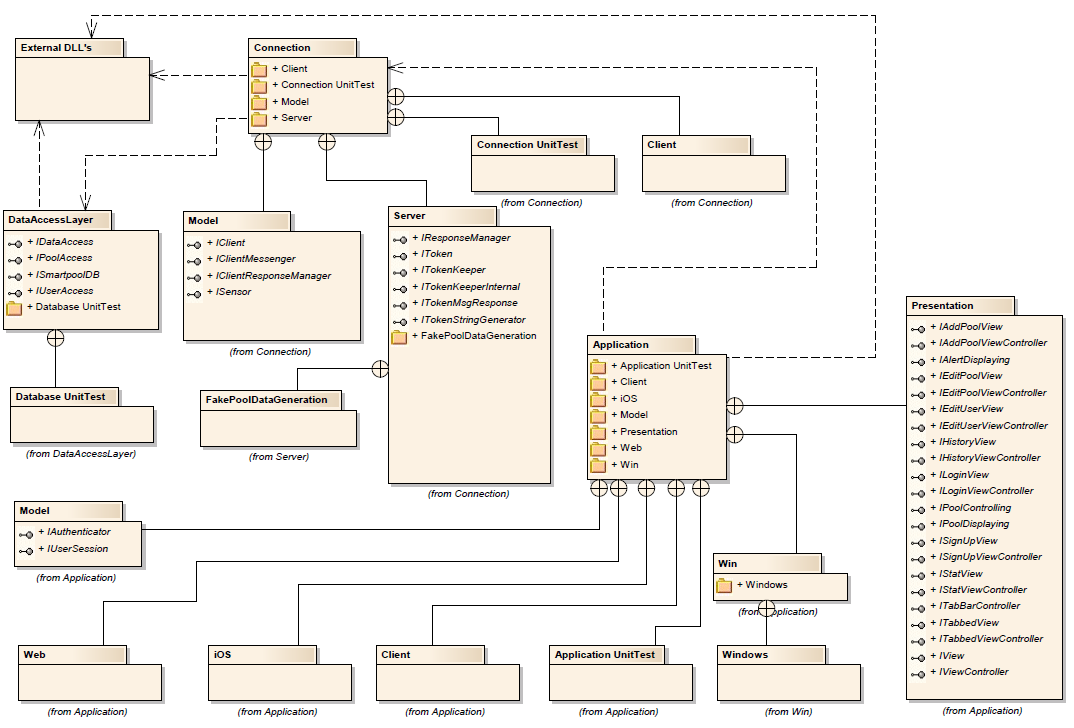
\includegraphics[width=\linewidth]{figs/arkitektur/packageDiagramNoImpl.PNG}
		\caption{Package model - Implementation/Development view}
		\label{fig:packageDiagram}
	\end{figure}
\end{landscape}
